\documentclass[10pt]{article}
\usepackage{fontspec}
\setmainfont{Latin Modern Roman}
\setmonofont{Latin Modern Mono}[Scale=0.9]
\usepackage[a4paper,margin=2cm]{geometry}
\usepackage{amssymb}
\usepackage{graphicx}
\usepackage{float}
\usepackage{booktabs}
\usepackage{tabularx}
\usepackage{array}
\usepackage{caption}
\usepackage{xcolor}
\usepackage[most]{tcolorbox}
\usepackage{microtype}
\usepackage{listings}
\lstset{basicstyle=\ttfamily\small,breaklines=true,breakatwhitespace=false,
  columns=fullflexible,backgroundcolor=\color{gray!8},frame=single,
  rulecolor=\color{gray!40},xleftmargin=4pt,xrightmargin=4pt,aboveskip=6pt,
  belowskip=6pt}
\usepackage{hyperref}
\hypersetup{colorlinks=true,linkcolor=blue!50!black,urlcolor=blue!50!black}
\newcolumntype{L}{>{\raggedright\arraybackslash}X}
\newtcolorbox{quotebox}{colback=gray!8,colframe=gray!40,boxrule=0.5pt,
  left=6pt,right=6pt,top=4pt,bottom=4pt,arc=2pt}
\setlength{\tabcolsep}{4pt}
\renewcommand{\arraystretch}{1.12}
\captionsetup{font=small,labelformat=empty}
\setlength{\parindent}{0pt}
\setlength{\parskip}{4pt}
\usepackage{sectsty}
\sectionfont{\large\bfseries\color{blue!30!black}}
\begin{document}
\begin{center}{\LARGE\bfseries Mega8 Simulation Analysis Report}\end{center}\vspace{6pt}

\section*{0. Executive summary}

Mega8 is the \textbf{first full balance sweep on the re-axed champion roster} (T.36b, merged to \texttt{main} via PR \#45) and the deepest to date: nine team sizes (2v2--10v10) $\times$ six weathers, 360 pieces (120 bases $\times$ 3 levels), with a combined median of \textbf{2{,}340 matches/piece} --- roughly 10$\times$ the per-cell depth of mega7. Because the roster shape is otherwise unchanged, the mega7$\rightarrow$mega8 deltas \textbf{isolate the re-axis}.\\

Five headline findings:\\

1. \textbf{Faction balance is sound.} Champion vs enemy win rate sits at 0.508 / 0.494 pooled and stays within $\pm$0.015 at every team size. Every residual below is \emph{within} the roster, not a champion/enemy asymmetry.\\

2. \textbf{The mage deficit is fixed.} This was the standing pathology in mega6/mega7 --- mages were the floor role with a sharp small-format within-tier deficit (+0.079 at 2v2). The re-axis closes it: the within-tier mage deficit flips to \textbf{$-$0.011 at 2v2} (a $-$0.089 swing), and mage pooled \texttt{wr\_\allowbreak{}delta} is now \textbf{+0.015} --- a mild \emph{surplus}. Mage win rate (0.522) now sits comfortably mid-pack.\\

3. \textbf{Role residuals are tight; apparent role spread is power-position, not mistuning.} Pooled win rates span support 0.459 to spellblade 0.565 ($\sim$10pp), but the pooled \texttt{wr\_\allowbreak{}delta} band is narrow (spellslinger $-$0.017 to mage +0.015). support (0.459) and tank (0.476) read low on raw win rate but their \texttt{wr\_\allowbreak{}delta} is $\approx$0 --- they are low-power-concentrated roles losing about what their power predicts, \emph{not} under-tuned kits.\\

4. \textbf{Apex L3 high-power pieces under-deliver vs their power budget --- the one open issue.} The new power-vs-budget boxplot (\S{}7) shows residuals flat on 0 through $P\!\le\!20$, then the top L3 band ($P$ 32--64) sags to $-$0.04\,--\,$-$0.05. By piece: \textbf{Aurion} (clear T10 L3, $-$0.151, the single worst piece), \textbf{Maw of the Drowned} ($-$0.131), \textbf{Hierarch} ($-$0.128), \textbf{Stone Warden} ($-$0.124). They win on raw power but less than their power says they should. Milder than mega7's $-$0.09 apex sag, but the same structural shape --- the candidate for a T.36c pass.\\

5. \textbf{Weather favor is modest and the metric is now clean.} Own-weather edge is \textbf{+0.013 own-vs-counter} and \textbf{+0.010 own-vs-clear}, positive for every affinity. The \texttt{counter\_\allowbreak{}weather\_\allowbreak{}wr} zero-fill artefact that overstated this in earlier sweeps is fully resolved --- \textbf{0.0\% of rows} now carry a spurious counter==0 (the buggy column-average and the raw computation agree: +0.012 vs +0.013).\\

\textbf{Two caveats lifted since mega7.} (a) \textbf{Timeouts no longer climb with team size} --- they hold flat at $\sim$9--11\% across all sizes (mega7 hit 44\% at 10v10), so large-format role reads are now trustworthy. (b) \textbf{Per-cell depth is no longer thin} (median 2{,}340 matches/piece), so per-stage win-rate spread is real signal rather than binomial noise.\\

\textbf{Three supplementary lenses (\S\S{}10--12).} A roster-health index (\S{}10) scores the sweep against the win-rate-band framework Riot uses for League of Legends: \textbf{84\% of pieces are within $\pm$0.05 of budget and only 2.8\% (10 pieces) beyond $\pm$0.10} --- a healthy roster by that standard. A combat-pacing pass (\S{}11) and an unsupervised behavioral-archetype clustering (\S{}12) then re-frame the apex sag: \textbf{it is a \emph{pacing} problem.} High-power pieces split into fast finishers and slow grinders, and the under-delivery lives almost entirely in the \emph{slow durable} apex archetype (wins by grinding toward the tick cap), not the fast finishers.\\

\section*{1. Dataset and method}

\medskip
\begin{tabularx}{\linewidth}{LL}
\toprule
\textbf{Field} & \textbf{Value} \\
\midrule
Directory & \texttt{results/\allowbreak{}mega/\allowbreak{}mega8/\allowbreak{}} \\
Run date & 2026-06-18 \\
Engine state & current working tree after the T.36b champion re-axis (PR \#45 merged): roster stat/playstyle rebalance \\
Stages & 2v2, 3v3, 4v4, 5v5, 6v6, 7v7, 8v8, 9v9, 10v10 (no 1v1) \\
Per-stage rated rows & 19,440 \\
Combined pieces & 360 (120 bases $\times$ 3 levels) \\
Weathers & clear, cloudy, mist, rain, snow, thunder \\
Median matches/piece (combined) & 2,340 \\
max-ticks & 12,000 (engine default --- sudden death engaged) \\
Baseline & mega7 (\texttt{cache\_\allowbreak{}mega7.\allowbreak{}rds}) \\
\bottomrule
\end{tabularx}
\medskip

\textbf{The combined file is the canonical aggregate.} \texttt{ratings\_\allowbreak{}combined.\allowbreak{}csv} pools every battle (pair-game weighted) across all stages and weathers, so its per-piece win rates and cross-weather metrics are the reliable read. All \S{}7--\S{}9 outlier work uses it.\\

\textbf{\texttt{wr\_\allowbreak{}delta} interpretation.} \texttt{expected\_\allowbreak{}wr} is the deterministic power-threshold model: 1.0 if your team's $\Sigma$P exceeds the opponent's, 0.0 if less, 0.5 if equal, averaged over the actual opponent field. \texttt{wr\_\allowbreak{}delta = win\_\allowbreak{}rate $-$ expected\_\allowbreak{}wr}. Near 0 = on-budget; negative = kit under-delivers vs power; positive = over-delivers. \texttt{expected\_\allowbreak{}power} is the T.18 scalar $P(T,L) = 2^{(T-1)/3 + \mathrm{triplings}(L)}$, $\mathrm{triplings}=\{$L1:0, L2:1, L3:3$\}$.\\

\section*{2. Aggregate balance}

\medskip
\begin{tabularx}{\linewidth}{Lrrrr}
\toprule
\textbf{stage} & \textbf{champion} & \textbf{enemy} & \textbf{sd(win\_rate)} & \textbf{timeout} \\
\midrule
2v2 & 0.507 & 0.496 & 0.195 & 0.110 \\
3v3 & 0.510 & 0.491 & 0.162 & 0.107 \\
4v4 & 0.509 & 0.492 & 0.150 & 0.087 \\
5v5 & 0.508 & 0.493 & 0.135 & 0.090 \\
6v6 & 0.505 & 0.498 & 0.134 & 0.089 \\
7v7 & 0.514 & 0.489 & 0.122 & 0.090 \\
8v8 & 0.506 & 0.496 & 0.121 & 0.089 \\
9v9 & 0.507 & 0.495 & 0.115 & 0.095 \\
10v10 & 0.505 & 0.495 & 0.114 & 0.085 \\
\bottomrule
\end{tabularx}
\medskip

Champion/enemy parity holds across all formats ($\pm$0.015). Win-rate spread declines smoothly with team size (0.195 $\rightarrow$ 0.114) as larger teams average individual variance out --- and because per-cell depth is now high, this is a \emph{real} effect, not the noise-inflated reading mega7 carried. \textbf{Timeouts stay flat at $\sim$9--11\% across all sizes} --- mega7's large-format timeout blow-up (44\% at 10v10) is gone, so every size resolves organically and role reads are comparable end-to-end.\\

\begin{figure}[H]\centering
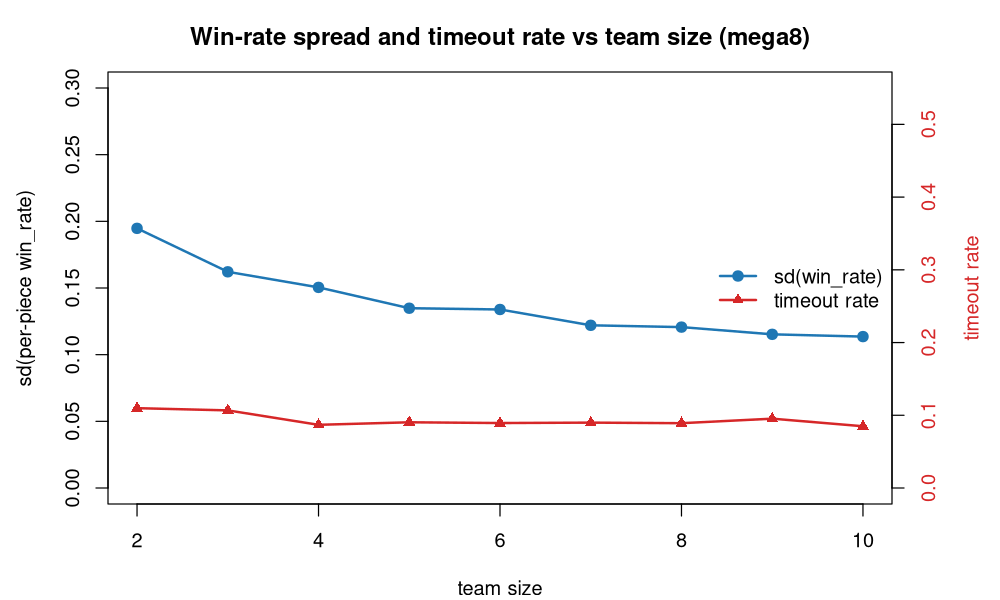
\includegraphics[width=0.86\linewidth,height=0.42\textheight,keepaspectratio]{plots/m8_02_variance_timeout_vs_size.png}
\caption*{\small win\_rate spread and timeout vs team size}
\end{figure}

\section*{3. Role balance}

\subsection*{3.1 Win rate by team size}

\begin{figure}[H]\centering
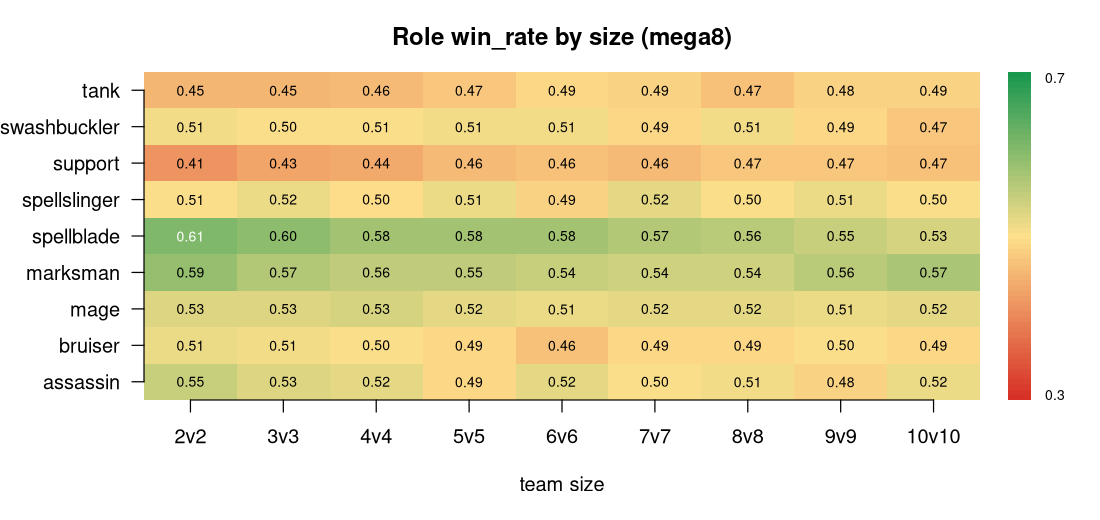
\includegraphics[width=0.86\linewidth,height=0.42\textheight,keepaspectratio]{plots/m8_04_role_wr_heatmap.png}
\caption*{\small Role win\_rate by size (heatmap)}
\end{figure}

Pooled (combined) role win rates:\\

\medskip
\begin{tabularx}{\linewidth}{Lr}
\toprule
\textbf{role} & \textbf{win\_rate} \\
\midrule
support & 0.459 \\
tank & 0.476 \\
bruiser & 0.492 \\
swashbuckler & 0.497 \\
spellslinger & 0.507 \\
assassin & 0.510 \\
mage & 0.522 \\
marksman & 0.557 \\
spellblade & 0.565 \\
\bottomrule
\end{tabularx}
\medskip

Spellblade and marksman are the ceiling; support and tank the floor. But raw win rate conflates kit tuning with where a role sits on the power curve --- see \S{}3.2.\\

\subsection*{3.2 Tuning residuals (wr\_delta)}

Pooled (combined) role \texttt{wr\_\allowbreak{}delta}:\\

\medskip
\begin{tabularx}{\linewidth}{Lr}
\toprule
\textbf{role} & \textbf{wr\_delta} \\
\midrule
spellslinger & $-$0.017 \\
bruiser & $-$0.011 \\
spellblade & $-$0.009 \\
tank & $-$0.006 \\
assassin & $-$0.003 \\
swashbuckler & +0.004 \\
support & +0.008 \\
marksman & +0.009 \\
mage & +0.015 \\
\bottomrule
\end{tabularx}
\medskip

\textbf{The residual band is narrow ($\pm$0.017) --- the roster is well-tuned against power.} The story splits from raw win rate: \textbf{support (0.459 raw) and tank (0.476 raw) carry $\approx$0 \texttt{wr\_\allowbreak{}delta}} --- they lose about what their (low) power predicts, so the low win rate is power-position, not mistuning. \textbf{spellblade has the second-highest raw win rate but a \emph{negative} residual ($-$0.009)} --- it wins on power, and front-loads: 0.61 at 2v2 decaying to 0.53 at 10v10 (small-team snowball). marksman and mage genuinely over-deliver on kit (+0.009/+0.015).\\

\begin{figure}[H]\centering
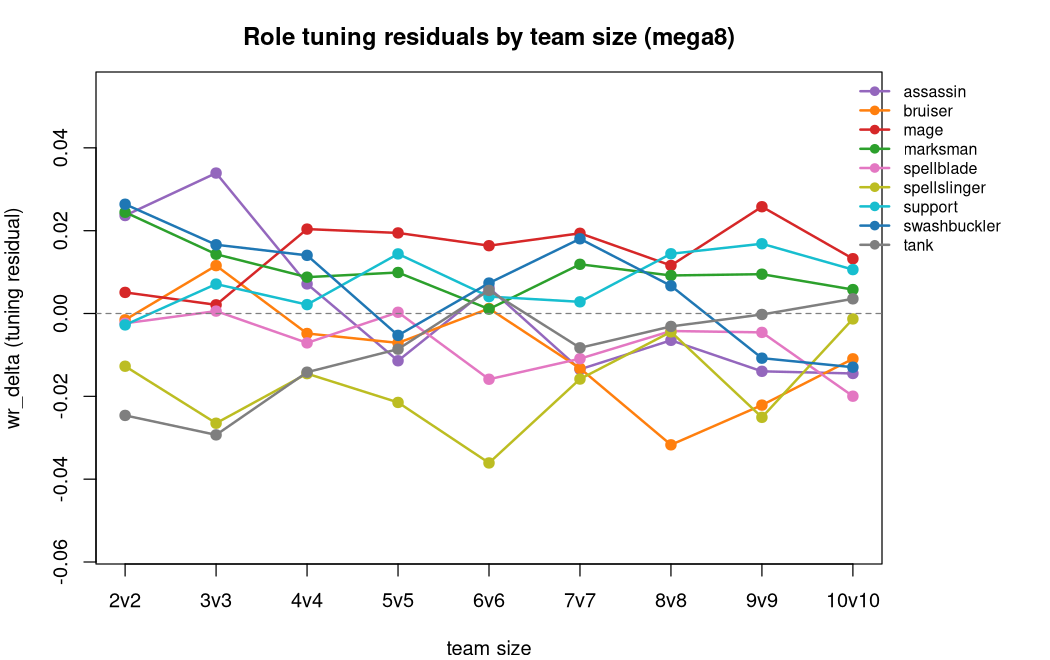
\includegraphics[width=0.86\linewidth,height=0.42\textheight,keepaspectratio]{plots/m8_01_role_wrdelta_vs_size.png}
\caption*{\small Role tuning residuals by team size}
\end{figure}

\section*{4. Mage deficit --- closed}

\medskip
\begin{tabularx}{\linewidth}{LrrLr}
\toprule
\textbf{stage} & \textbf{mage} & \textbf{nonmage} & \textbf{within\_tier\_def} & \textbf{cor(tier,wr)} \\
\midrule
2v2 & 0.529 & 0.497 & $-$0.011 & 0.555 \\
3v3 & 0.527 & 0.497 & $-$0.016 & 0.538 \\
4v4 & 0.535 & 0.495 & $-$0.014 & 0.499 \\
5v5 & 0.523 & 0.498 & $-$0.005 & 0.487 \\
6v6 & 0.513 & 0.500 & +0.002 & 0.430 \\
7v7 & 0.522 & 0.499 & $-$0.009 & 0.462 \\
8v8 & 0.522 & 0.498 & $-$0.013 & 0.460 \\
9v9 & 0.513 & 0.499 & +0.005 & 0.406 \\
10v10 & 0.519 & 0.498 & $-$0.001 & 0.457 \\
\bottomrule
\end{tabularx}
\medskip

The within-tier mage deficit is gone at every size --- mages now sit at or slightly above their tier cohort throughout. Against mega7 at matched sizes the swing is decisive at small formats:\\

\medskip
\begin{tabularx}{\linewidth}{Lrrr}
\toprule
\textbf{stage} & \textbf{mega7 deficit} & \textbf{mega8 deficit} & \textbf{$\Delta$} \\
\midrule
2v2 & +0.079 & $-$0.011 & $-$0.089 \\
3v3 & +0.011 & $-$0.016 & $-$0.027 \\
4v4 & +0.019 & $-$0.014 & $-$0.033 \\
5v5 & +0.045 & $-$0.005 & $-$0.050 \\
6v6 & +0.034 & +0.002 & $-$0.032 \\
10v10 & +0.023 & $-$0.001 & $-$0.024 \\
\bottomrule
\end{tabularx}
\medskip

(Positive = mages behind their tier; a negative $\Delta$ = improvement.) The re-axis targeted exactly the small-format weakness and landed it. A handful of individual mages still read under power (Steam Engineer T4 L3 $-$0.114, Drowned Siren T4 L3 $-$0.079) but these are now ordinary tail pieces, not a role-wide floor.\\

\begin{figure}[H]\centering
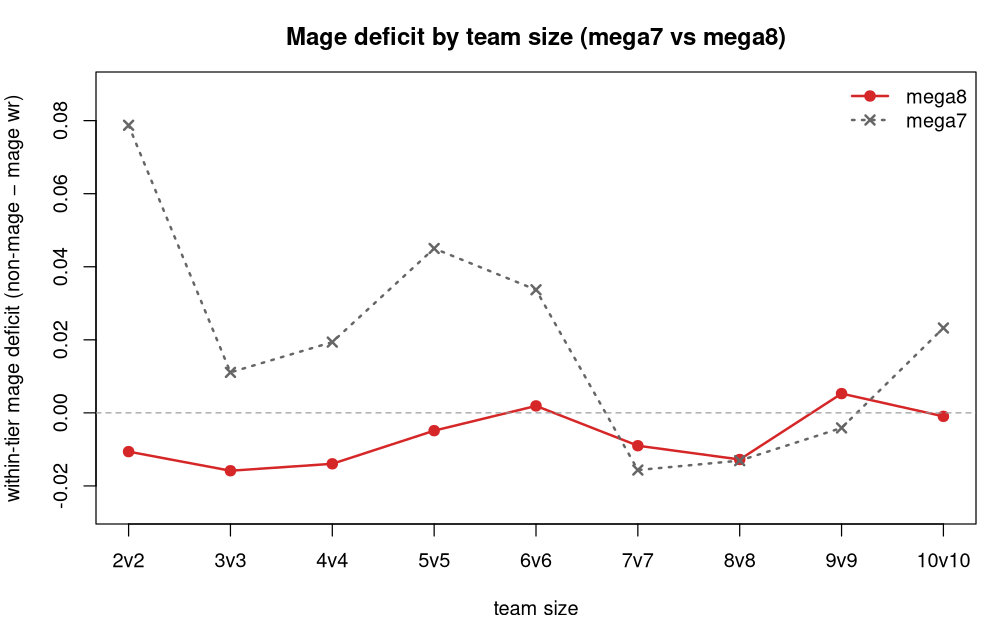
\includegraphics[width=0.86\linewidth,height=0.42\textheight,keepaspectratio]{plots/m8_03_mage_deficit_by_size.png}
\caption*{\small Mage deficit by team size: mega7 vs mega8}
\end{figure}

\begin{figure}[H]\centering
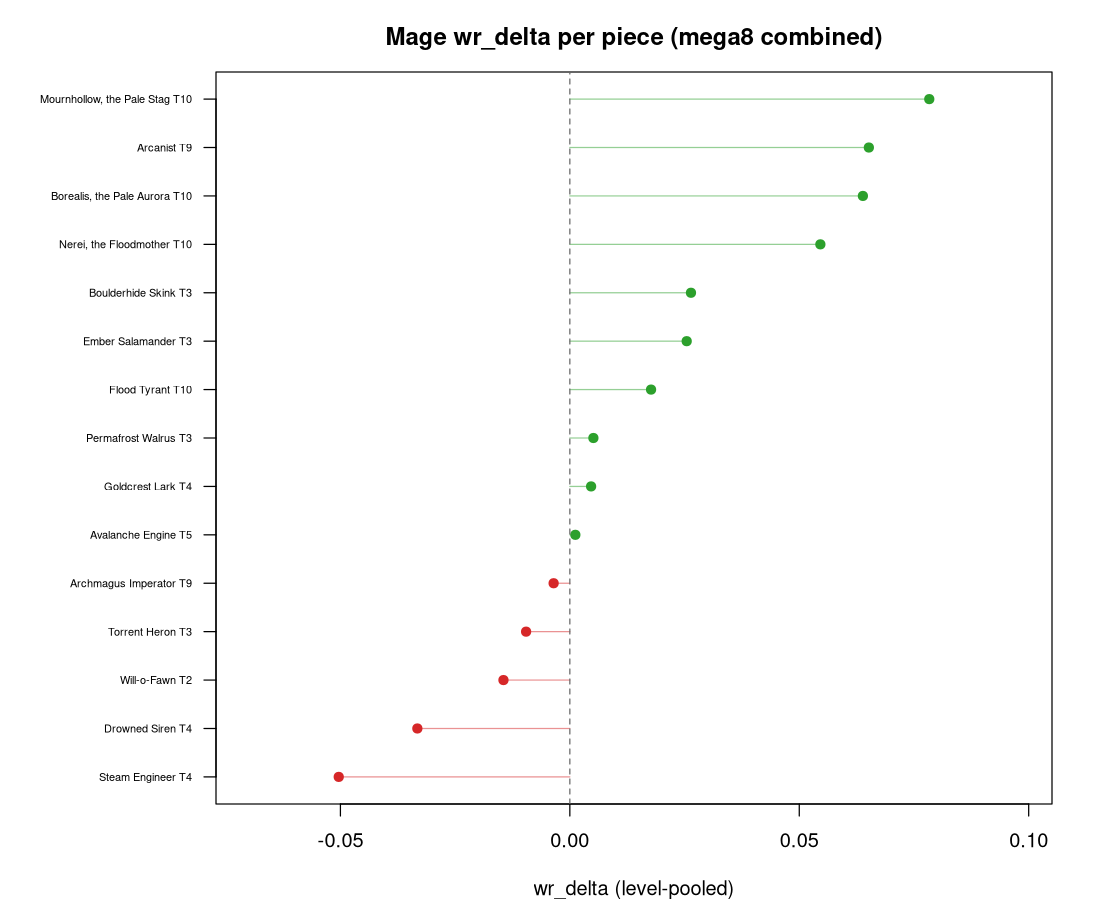
\includegraphics[width=0.86\linewidth,height=0.42\textheight,keepaspectratio]{plots/m8_08_mage_wrdelta.png}
\caption*{\small Mage wr\_delta per piece (combined)}
\end{figure}

\section*{5. Level effects}

\medskip
\begin{tabularx}{\linewidth}{rrLr}
\toprule
\textbf{level} & \textbf{win\_rate} & \textbf{wr\_delta} & \textbf{timeout} \\
\midrule
1 & 0.427 & +0.011 & 0.092 \\
2 & 0.468 & +0.008 & 0.095 \\
3 & 0.608 & $-$0.017 & 0.098 \\
\bottomrule
\end{tabularx}
\medskip

The level premium is steep (L1$\rightarrow$L3 = +0.18 raw) but \texttt{wr\_\allowbreak{}delta} stays small: L1/L2 slightly over-deliver, \textbf{L3 slightly \emph{under}-delivers ($-$0.017)}. That L3 sag is the level-axis shadow of the apex-power issue in \S{}7 --- the highest-power state is where kits stop fully converting power into wins. By design otherwise; no broad action needed.\\

\begin{figure}[H]\centering
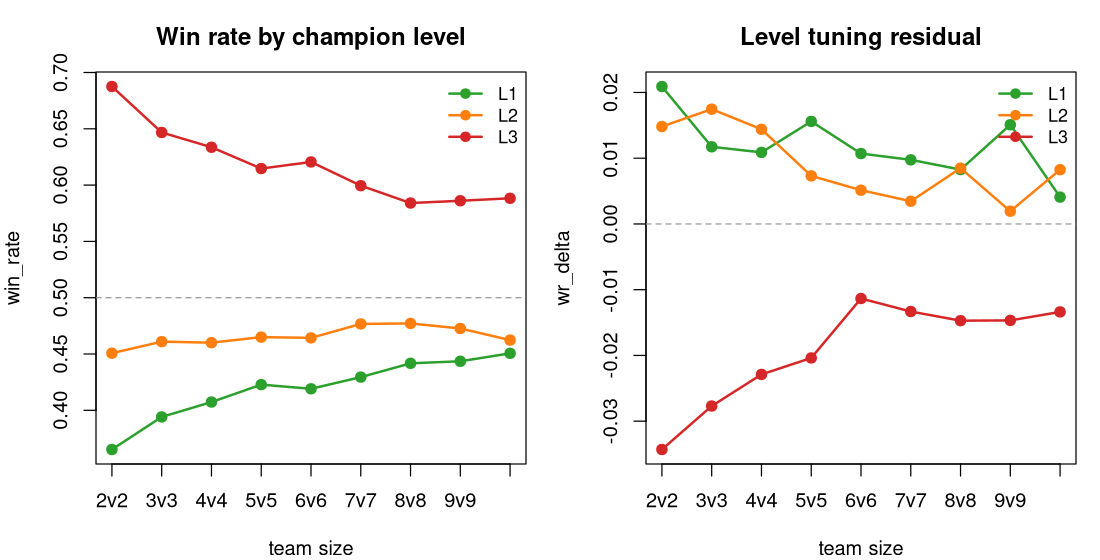
\includegraphics[width=0.86\linewidth,height=0.42\textheight,keepaspectratio]{plots/m8_05_level_effect.png}
\caption*{\small Win rate and tuning residual by champion level}
\end{figure}

\section*{6. Weather effects}

Own-weather advantage is real, positive for every affinity, and \textbf{modest ($\sim$+0.01)}. The \texttt{counter\_\allowbreak{}weather\_\allowbreak{}wr} zero-fill artefact that overstated weather favor in earlier sweeps is now fully resolved: \textbf{counter==0 fires in 0.0\% of rows}, so the buggy column-average (+0.012) and the correct raw computation (+0.013) agree.\\

\textbf{Own-weather advantage by size} (own = win rate in own affinity weather; clear = no-favor baseline; counter = weather that preys on you):\\

\medskip
\begin{tabularx}{\linewidth}{Lrrrrr}
\toprule
\textbf{stage} & \textbf{clear (base)} & \textbf{own} & \textbf{counter} & \textbf{own $-$ counter} & \textbf{own $-$ clear} \\
\midrule
2v2 & 0.500 & 0.514 & 0.496 & +0.017 & +0.014 \\
4v4 & 0.500 & 0.510 & 0.499 & +0.011 & +0.010 \\
6v6 & 0.500 & 0.510 & 0.495 & +0.016 & +0.010 \\
8v8 & 0.500 & 0.508 & 0.499 & +0.009 & +0.008 \\
10v10 & 0.500 & 0.507 & 0.493 & +0.014 & +0.007 \\
\bottomrule
\end{tabularx}
\medskip

\textbf{Per-affinity} (raw, pooled all stages):\\

\medskip
\begin{tabularx}{\linewidth}{Lrrrrr}
\toprule
\textbf{affinity} & \textbf{clear} & \textbf{own} & \textbf{counter} & \textbf{own $-$ clear} & \textbf{own $-$ counter} \\
\midrule
mist & 0.521 & 0.526 & 0.506 & +0.005 & +0.020 \\
cloudy & 0.505 & 0.524 & 0.492 & +0.019 & +0.032 \\
rain & 0.500 & 0.519 & 0.496 & +0.018 & +0.023 \\
snow & 0.516 & 0.527 & 0.499 & +0.011 & +0.028 \\
thunder & 0.497 & 0.517 & 0.490 & +0.020 & +0.027 \\
\bottomrule
\end{tabularx}
\medskip

Every affinity gains in its own weather and loses (or is flat) in its counter --- the favor system works as designed. The magnitude is single-digit win-rate points, so weather is a flavour-and-edge axis, not a dominant one. Sensitivity (per-piece spread of per-weather win rate) rises gently with team size (0.056 at 2v2 $\rightarrow$ 0.079 at 10v10), as more pieces share the same weather field.\\

\begin{figure}[H]\centering
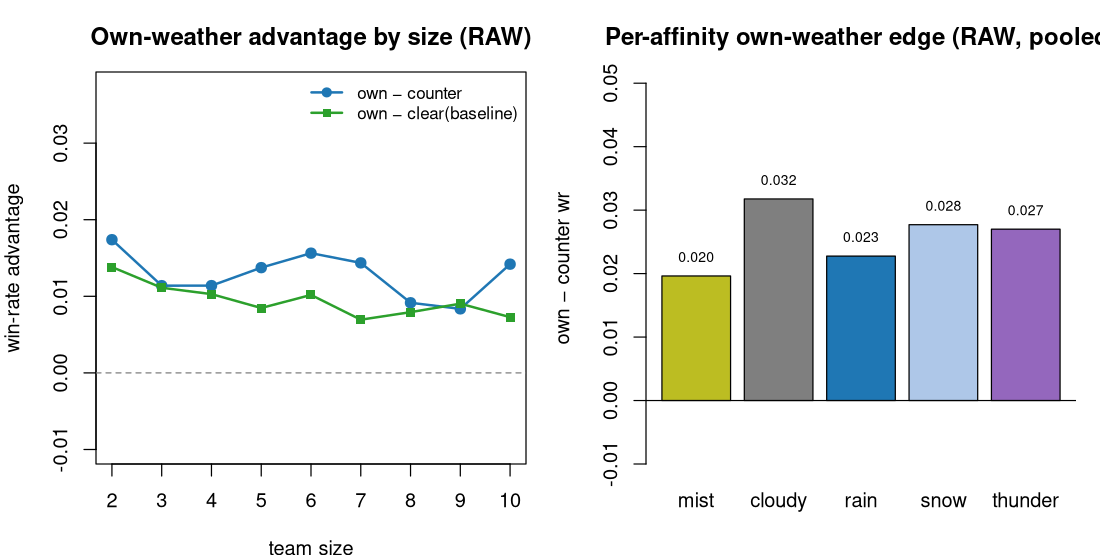
\includegraphics[width=0.86\linewidth,height=0.42\textheight,keepaspectratio]{plots/m8_06_weather_effects.png}
\caption*{\small Weather: own-advantage by size and per-affinity edge}
\end{figure}

\section*{7. Power vs budget --- the apex sag}

This sweep adds a per-piece view of win rate against the power scalar that drives \texttt{expected\_\allowbreak{}wr}. Because mega8 draws teams at random, high-power pieces routinely meet low-power ones, so \textbf{win\_rate \emph{should} climb with power} --- that climb is the deterministic power model working, not a finding. The diagnostic is the \emph{residual}: \texttt{wr\_\allowbreak{}delta} after the power curve is removed should sit flat on 0 at every power level. Each box is one distinct \texttt{expected\_\allowbreak{}power}; the 30 (tier,level) combinations collapse to 19 distinct powers because $P(T,L)$ interleaves tier and level (e.g. T3/L1 $=$ T1/L2 $=$ 2.0).\\

\begin{figure}[H]\centering
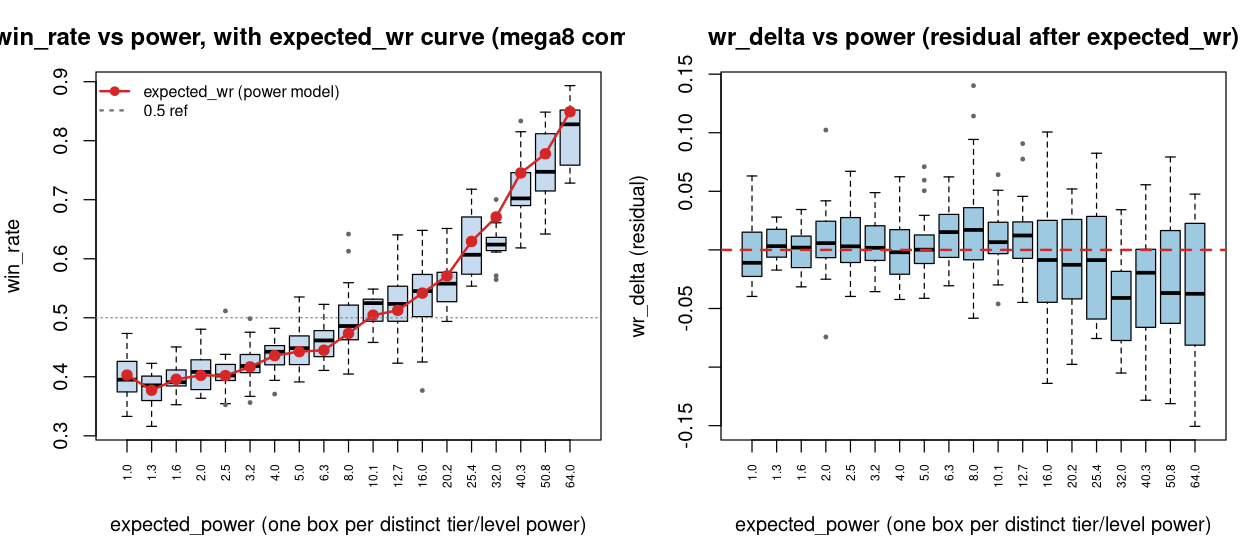
\includegraphics[width=0.96\linewidth,height=0.44\textheight,keepaspectratio]{plots/m8_12_wr_vs_power.png}
\caption*{\small Left: win\_rate per power bin with the expected\_wr curve overlaid (boxes track the curve). Right: wr\_delta residual per power bin (flat on 0 = tuned).}
\end{figure}

\textbf{Reading.} The left panel's boxes hug the red \texttt{expected\_\allowbreak{}wr} curve --- the power model predicts win rate well across the whole range. The right panel is flat on 0 through $P\!\le\!20$ (residuals slightly positive, $\sim$+0.01--0.02, through the mid-band), then \textbf{the top L3 band ($P$ = 32, 40, 51, 64) sags negative ($-$0.04 to $-$0.05) with wide boxes}. That is the apex sag: the highest-power pieces under-convert their raw power into wins. It is milder than mega7 ($-$0.09) but structurally identical, and it lines up with the L3 residual in \S{}5 --- the issue is the \emph{apex L3 state}, not any one tier.\\

\textbf{Named fliers (1.5$\times$IQR).} R draws boxplot outliers as unlabelled dots; these are the pieces deviating most from their \emph{power cohort} (others at the same $P$), so they are the prime within-power tuning candidates. A flier is mechanically a piece beyond 1.5$\times$IQR of its cohort; the \emph{read} column says what that deviation likely means. Recurring patterns (tags used in all four flier tables):\\

\begin{quotebox}
\textbf{AG --- apex grinder:} high-power L3 in a durable/slow kit; wins on raw stats but stalls toward the tick cap, so it under-converts power (\S{}11--12). \emph{Fix: closing/burst, not stats.}\quad
\textbf{EB --- early bloomer:} low-tier (T1--3) kit stronger than its power band; over-delivers. \emph{Fix: trim early scaling.}\quad
\textbf{DA --- dead apex:} an L3 piece that also loses on \emph{raw} win rate --- kit barely converts at all. \emph{Fix: damage/survivability.}\quad
\textbf{CH --- cohort split:} win\_rate far from same-power peers (a role$\times$power mismatch).\quad
\textbf{LF --- level-flip:} over-budget at one level, under at another (mis-shaped level scaling).
\end{quotebox}
\medskip

\textit{win\_rate panel --- deviates from cohort win rate at the same power.} The \textbf{cohort} column gives the box's min\,/\,mean\,/\,max win rate \emph{excluding the fliers} (i.e. the whisker range and body mean), so every flier here sits \emph{outside} its [min, max] --- the gap shows how far:\\
{\small
\begin{tabularx}{\linewidth}{rlrlL}
\toprule
$P$ & \textbf{piece} (role) & \textbf{wr} & \textbf{cohort min/$\mu$/max} & \textbf{why a flier / what it could mean} \\
\midrule
2.5 & Frostplate Tortoise T5/L1 (tank) & 0.352 & .35\,/\,.41\,/\,.44 & CH-low --- below the box; a tank at low power loses more than its peers, durability buys little when base stats are small. \\
2.5 & Veldt Pronghorn T2/L2 (tank) & 0.511 & .35\,/\,.41\,/\,.44 & CH-high --- above the box; over-performs the low-$P$ field. \\
3.2 & Hollowed Wisp T3/L2 (assassin) & 0.356 & .37\,/\,.42\,/\,.48 & CH-low --- below the box; fragile assassin folds before it can burst. \\
3.2 & Iron-Collared Hound T3/L2 (swash) & 0.498 & .37\,/\,.42\,/\,.48 & CH-high --- above the box; wins more than its P3.2 peers. \\
4.0 & Drowned Siren T4/L2 (mage) & 0.371 & .39\,/\,.44\,/\,.48 & CH-low / early under --- below the box; mid mage under-delivers. \\
8.0 & Borealis T10/L1 (mage) & 0.613 & .41\,/\,.49\,/\,.56 & CH-high --- above the box; a T10 king already beats its P8 peers at L1. \\
8.0 & Springfrog T1/L3 (support) & 0.642 & .41\,/\,.49\,/\,.56 & EB --- above the box; a T1 piece winning 64\% at P8 is over-scaled for its tier. \\
16 & Steam Engineer T4/L3 (mage) & 0.377 & .43\,/\,.54\,/\,.65 & DA --- far below the box; an L3 mage $\sim$16pp under its peers' mean, kit not converting. \\
32 & Mirewarden Toad T7/L3 (tank) & 0.565 & .61\,/\,.63\,/\,.66 & AG (CH-low) --- below the box; apex tank grinds. \\
32 & Marshghast Boar T7/L3 (bruiser) & 0.571 & .61\,/\,.63\,/\,.66 & AG (CH-low) --- below the box; apex bruiser stalls. \\
32 & Thunder Bull T7/L3 (support) & 0.700 & .61\,/\,.63\,/\,.66 & CH-high --- above the box; unusually strong apex support for P32. \\
40 & Glade Heron T8/L3 (marksman) & 0.833 & .62\,/\,.71\,/\,.82 & CH-high --- above the box / top apex finisher; wins big but on-budget (fast, not a grinder). \\
\bottomrule
\end{tabularx}
}
\medskip

\textit{wr\_delta panel --- residual after the power curve is removed} (cohort = box min\,/\,mean\,/\,max \emph{excluding fliers}; every flier sits outside it):\\
{\small
\begin{tabularx}{\linewidth}{rlrlL}
\toprule
$P$ & \textbf{piece} (role) & \textbf{$\Delta$} & \textbf{cohort min/$\mu$/max} & \textbf{why a flier / what it could mean} \\
\midrule
2.0 & Conscript T1/L2 (swash) & $-$0.074 & $-$.03/+.01/+.04 & Early under --- below the box; weak starter kit even after adjusting for power. \\
2.0 & Springfrog T1/L2 (support) & +0.102 & $-$.03/+.01/+.04 & EB --- above the box; over-budget at T1 already. \\
5.0 & Coral Colossus T5/L2 (tank) & +0.051 & $-$.04/$-$.01/+.03 & Over --- above the box; tank punching above its P5 budget. \\
5.0 & Hierarch T8/L1 (support) & +0.059 & $-$.04/$-$.01/+.03 & LF --- above the box; Hierarch is \emph{over} at L1 but the worst apex \emph{under} at L3: level scaling mis-shaped. \\
5.0 & Caged Banshee T5/L2 (support) & +0.071 & $-$.04/$-$.01/+.03 & Over --- above the box; mid support above budget. \\
8.0 & Borealis T10/L1 (mage) & +0.114 & $-$.06/+.02/+.09 & Over --- above the box; king kit already over-budget at L1. \\
8.0 & Springfrog T1/L3 (support) & +0.140 & $-$.06/+.02/+.09 & EB --- above the box and the largest positive residual in the sweep; clearest over-scaled low-tier kit. \\
10 & Powder Sapper T2/L3 (support) & $-$0.046 & $-$.03/+.01/+.05 & Under --- below the box; a low-tier L3 support that lags. \\
10 & Veilfang Wolf T8/L2 (swash) & +0.064 & $-$.03/+.01/+.05 & Over --- above the box; swashbuckler above budget. \\
13 & Ember Salamander T3/L3 (mage) & +0.077 & $-$.05/+.01/+.05 & EB --- above the box; low-tier mage over its budget. \\
13 & Arcanist T9/L2 (mage) & +0.091 & $-$.05/+.01/+.05 & Over --- above the box; high-tier mage above budget (a healthy over-performer). \\
\bottomrule
\end{tabularx}
}
\medskip

\section*{8. Timeouts}

\medskip
\begin{tabularx}{\linewidth}{Lrrrr}
\toprule
\textbf{role} & \textbf{2v2} & \textbf{5v5} & \textbf{8v8} & \textbf{10v10} \\
\midrule
assassin & 0.047 & 0.078 & 0.076 & 0.091 \\
bruiser & 0.142 & 0.100 & 0.104 & 0.097 \\
mage & 0.056 & 0.074 & 0.081 & 0.067 \\
marksman & 0.048 & 0.061 & 0.065 & 0.070 \\
support & 0.162 & 0.100 & 0.094 & 0.087 \\
tank & 0.191 & 0.126 & 0.109 & 0.103 \\
\bottomrule
\end{tabularx}
\medskip

\textbf{The mega7 timeout blow-up is gone.} Timeouts no longer climb with team size --- they peak at small formats for the durable low-burst roles (tank 0.19, support 0.16, bruiser 0.14 at 2v2, where two tanky pieces can grind past the cap) and fall as team size rises. At no size does any role approach mega7's 40\%+ stalls. Large-format role reads are now trustworthy.\\

\section*{9. Outliers and tuning priorities}

\subsection*{9.1 Distribution shape}

\begin{figure}[H]\centering
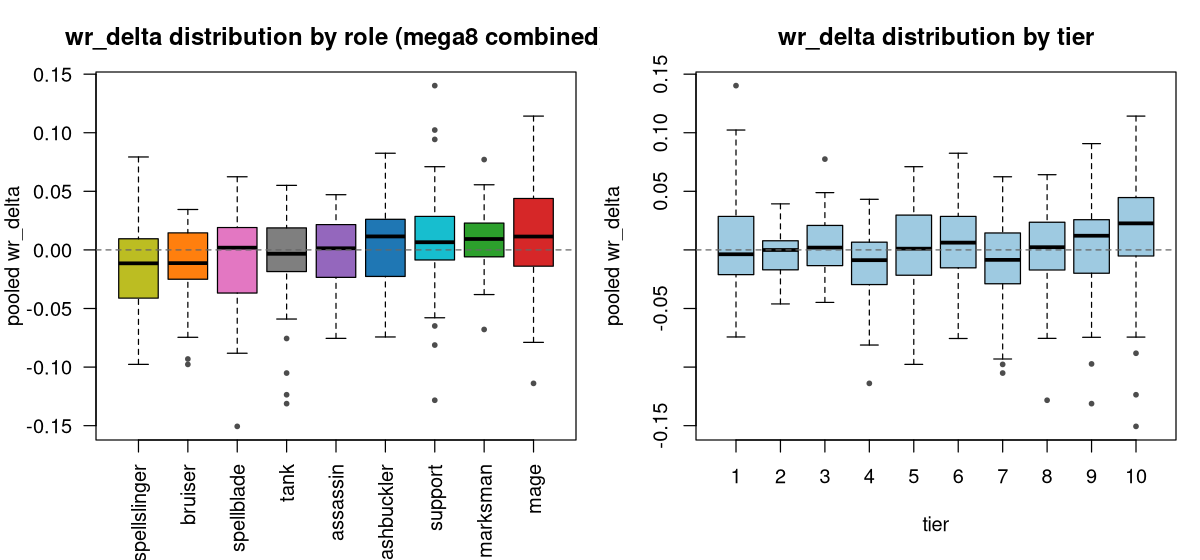
\includegraphics[width=0.86\linewidth,height=0.42\textheight,keepaspectratio]{plots/m8_09_wrdelta_boxplots.png}
\caption*{\small wr\_delta distribution by role and by tier (boxplots)}
\end{figure}

\textbf{Named fliers (1.5$\times$IQR) for both boxplots} (tags as defined in \S{}7). The unlabelled dots above, recovered --- the pieces most out of line with their \emph{role} cohort and their \emph{tier} cohort. These are the same names that dominate \S{}9.2, now attributed to the cohort that flags them.\\

\textit{by role --- residual vs others in the same role} (cohort = the role box's min\,/\,mean\,/\,max \emph{excluding fliers}):\\
{\small
\begin{tabularx}{\linewidth}{llrlL}
\toprule
\textbf{role} & \textbf{piece} & \textbf{$\Delta$} & \textbf{cohort min/$\mu$/max} & \textbf{why a flier / what it could mean} \\
\midrule
bruiser & Dredge-Hulk T7/L3 & $-$0.098 & $-$.08/$-$.01/+.04 & AG --- below the box; apex bruiser stalls toward the cap. \\
bruiser & Marshghast Boar T7/L3 & $-$0.093 & $-$.08/$-$.01/+.04 & AG --- below the box; second apex bruiser grinder. \\
mage & Steam Engineer T4/L3 & $-$0.114 & $-$.08/+.02/+.11 & DA --- below the box; worst mage, loses on raw win rate too. \\
marksman & Voltaic Diviner T5/L3 & $-$0.068 & $-$.04/+.01/+.06 & Under --- below the box; apex marksman lagging an over-budget role. \\
marksman & Umbra T10/L1 & +0.077 & $-$.04/+.01/+.06 & Over --- above the box; king over-budget at L1. \\
spellblade & Aurion T10/L3 & $-$0.151 & $-$.09/.00/+.06 & AG --- well below the box; the single worst piece in the sweep, apex king that grinds. \\
support & Hierarch T8/L3 & $-$0.128 & $-$.06/+.01/+.07 & AG --- below the box; on-death barrier helps allies not itself. \\
support & Coppercrest Stork T4/L3 & $-$0.081 & $-$.06/+.01/+.07 & Under --- below the box; mid support lagging its role. \\
support & Hoarfrost Owl T4/L3 & $-$0.065 & $-$.06/+.01/+.07 & Under --- below the box; mid support lagging its role. \\
support & Lostlight Wisp T1/L3 & +0.094 & $-$.06/+.01/+.07 & EB --- above the box; over-scaled T1 support. \\
support & Springfrog T1/L2 & +0.102 & $-$.06/+.01/+.07 & EB --- above the box; over-scaled T1 support. \\
support & Springfrog T1/L3 & +0.140 & $-$.06/+.01/+.07 & EB --- well above the box; T1 kit far above its band. \\
tank & Maw of the Drowned T9/L3 & $-$0.131 & $-$.06/.00/+.06 & AG --- below the box; durable apex tank wins by grinding. \\
tank & Stone Warden T10/L3 & $-$0.124 & $-$.06/.00/+.06 & AG --- below the box; apex tank grinder. \\
tank & Mirewarden Toad T7/L3 & $-$0.105 & $-$.06/.00/+.06 & AG --- below the box; apex tank grinder. \\
tank & Inquisitor T6/L3 & $-$0.076 & $-$.06/.00/+.06 & AG --- below the box; milder apex tank grinder. \\
\bottomrule
\end{tabularx}
}
\medskip

\textit{by tier --- residual vs others in the same tier} (cohort = the tier box's min\,/\,mean\,/\,max \emph{excluding fliers}):\\
{\small
\begin{tabularx}{\linewidth}{llrlL}
\toprule
\textbf{tier} & \textbf{piece} (role) & \textbf{$\Delta$} & \textbf{cohort min/$\mu$/max} & \textbf{why a flier / what it could mean} \\
\midrule
1 & Springfrog (support) & +0.140 & $-$.07/.00/+.10 & EB --- above the box; T1 kit over-scaled, the strongest piece vs its tier. \\
3 & Ember Salamander (mage) & +0.077 & $-$.05/.00/+.05 & EB --- above the box; low-tier mage above its tier cohort. \\
4 & Steam Engineer (mage) & $-$0.114 & $-$.08/$-$.01/+.04 & DA --- below the box; breaks below T4 and loses raw; kit under-built. \\
7 & Mirewarden Toad (tank) & $-$0.105 & $-$.09/$-$.01/+.06 & AG --- below the box; apex grinder, worst of its tier. \\
7 & Dredge-Hulk (bruiser) & $-$0.098 & $-$.09/$-$.01/+.06 & AG --- below the box; apex grinder, drags T7. \\
8 & Hierarch (support) & $-$0.128 & $-$.08/+.01/+.06 & AG --- below the box; apex grinder, worst of T8. \\
9 & Maw of the Drowned (tank) & $-$0.131 & $-$.08/+.01/+.09 & AG --- below the box; apex grinder, worst of T9. \\
9 & Cliffeyrie Eagle (sslinger) & $-$0.097 & $-$.08/+.01/+.09 & AG --- below the box; spellslinger that stalls at apex. \\
10 & Aurion (spellblade) & $-$0.151 & $-$.07/+.03/+.11 & AG --- well below the box; apex king, worst of T10 and the sweep. \\
10 & Stone Warden (tank) & $-$0.124 & $-$.07/+.03/+.11 & AG --- below the box; apex tank king, drags T10. \\
10 & Aerion (spellblade) & $-$0.088 & $-$.07/+.03/+.11 & AG --- below the box; second apex spellblade king grinder. \\
\bottomrule
\end{tabularx}
}
\medskip

\begin{figure}[H]\centering
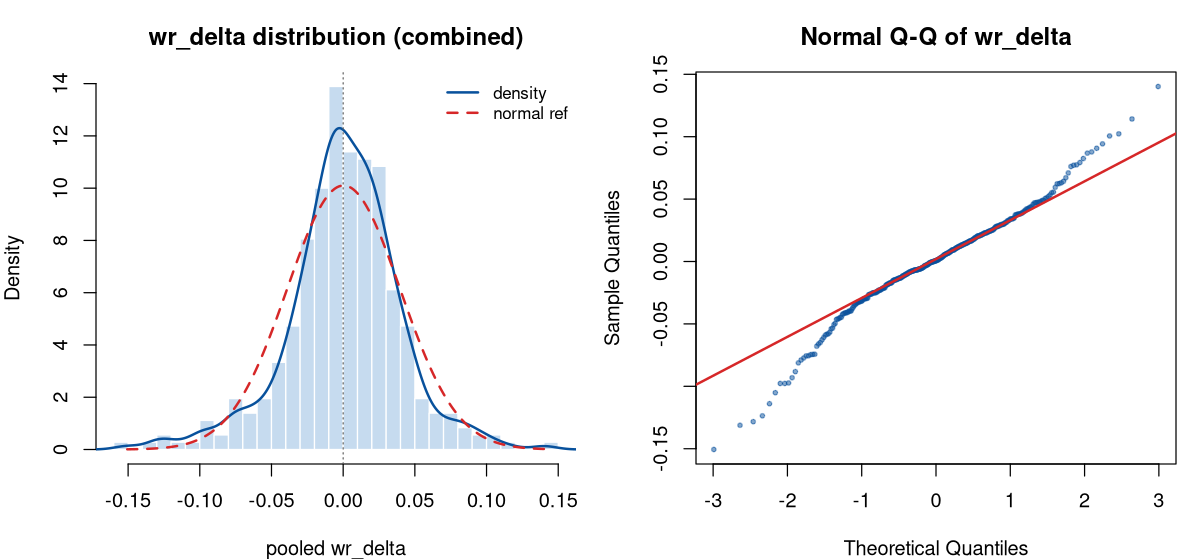
\includegraphics[width=0.86\linewidth,height=0.42\textheight,keepaspectratio]{plots/m8_10_wrdelta_distribution.png}
\caption*{\small wr\_delta distribution: histogram + density vs normal, and normal Q-Q}
\end{figure}

The pooled \texttt{wr\_\allowbreak{}delta} distribution is near-normal in the body and only mildly heavy-tailed --- most pieces sit within $\pm$0.08 of budget. By tier the boxes are tight and centred near 0 except the \textbf{T10 box, which skews negative} (the apex sag of \S{}7). The named outliers below are genuine within-tier tail events (\texttt{wd\_\allowbreak{}z} column), not a fat-tailed mess.\\

\subsection*{9.2 Absolute outliers (largest |wr\_delta|)}

\texttt{wd\_\allowbreak{}z} = within-tier z-score of \texttt{wr\_\allowbreak{}delta}. |z| $\gtrsim$ 2 $\approx$ a genuine per-tier outlier.\\

\begin{figure}[H]\centering
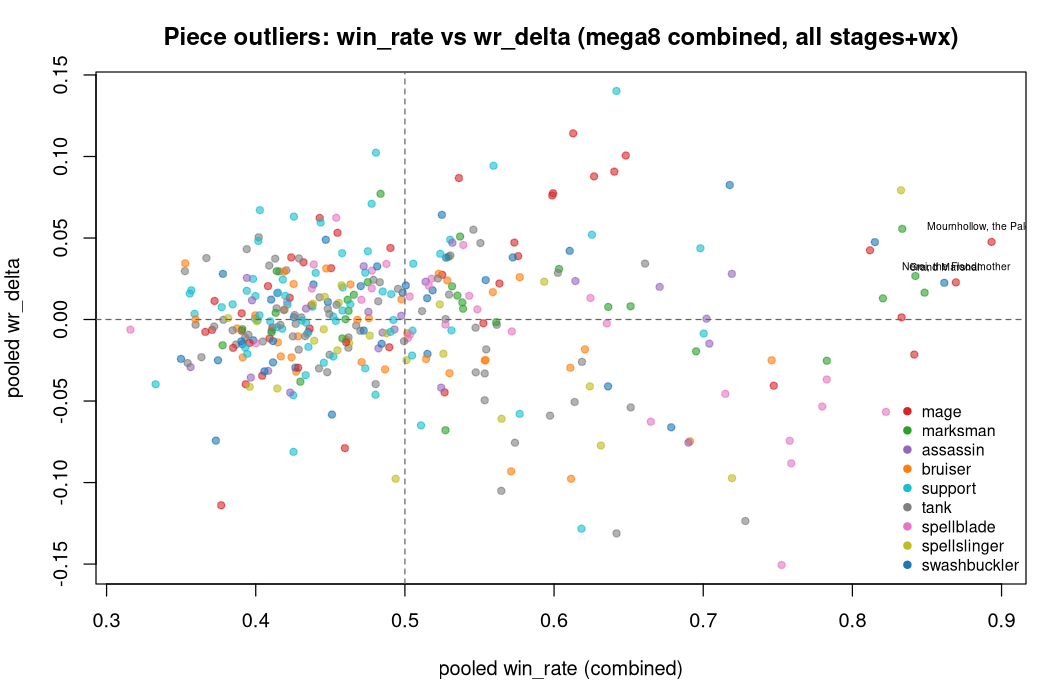
\includegraphics[width=0.86\linewidth,height=0.42\textheight,keepaspectratio]{plots/m8_07_outlier_scatter.png}
\caption*{\small Piece outliers: win\_rate vs wr\_delta (combined)}
\end{figure}

\textbf{Most under-tuned (pooled \texttt{wr\_\allowbreak{}delta}):}\\

\medskip
\begin{tabularx}{\linewidth}{LLLrrrrr}
\toprule
\textbf{name} & \textbf{affinity} & \textbf{role} & \textbf{tier} & \textbf{level} & \textbf{win\_rate} & \textbf{wr\_delta} & \textbf{wd\_z} \\
\midrule
Aurion, the First Dawn & clear & spellblade & 10 & 3 & 0.753 & $-$0.151 & $-$2.81 \\
Maw of the Drowned & rain & tank & 9 & 3 & 0.642 & $-$0.131 & $-$2.95 \\
Hierarch & clear & support & 8 & 3 & 0.618 & $-$0.128 & $-$2.96 \\
Stone Warden & cloudy & tank & 10 & 3 & 0.728 & $-$0.124 & $-$2.35 \\
Steam Engineer & clear & mage & 4 & 3 & 0.377 & $-$0.114 & $-$3.00 \\
Mirewarden Toad & rain & tank & 7 & 3 & 0.565 & $-$0.105 & $-$2.47 \\
Battlemage & clear & spellslinger & 5 & 3 & 0.494 & $-$0.098 & $-$2.78 \\
Dredge-Hulk & rain & bruiser & 7 & 3 & 0.611 & $-$0.098 & $-$2.27 \\
Cliffeyrie Eagle & cloudy & spellslinger & 9 & 3 & 0.719 & $-$0.097 & $-$2.20 \\
Marshghast Boar & mist & bruiser & 7 & 3 & 0.571 & $-$0.093 & $-$2.15 \\
\bottomrule
\end{tabularx}
\medskip

\textbf{Most over-tuned:}\\

\medskip
\begin{tabularx}{\linewidth}{LLLrrrrr}
\toprule
\textbf{name} & \textbf{affinity} & \textbf{role} & \textbf{tier} & \textbf{level} & \textbf{win\_rate} & \textbf{wr\_delta} & \textbf{wd\_z} \\
\midrule
Springfrog & rain & support & 1 & 3 & 0.642 & +0.140 & +2.91 \\
Borealis, the Pale Aurora & snow & mage & 10 & 1 & 0.613 & +0.114 & +1.72 \\
Springfrog & rain & support & 1 & 2 & 0.481 & +0.102 & +2.08 \\
Mournhollow, the Pale Stag & mist & mage & 10 & 2 & 0.648 & +0.101 & +1.49 \\
Lostlight Wisp & mist & support & 1 & 3 & 0.559 & +0.094 & +1.90 \\
Arcanist & clear & mage & 9 & 2 & 0.640 & +0.091 & +1.98 \\
Iceclaw Lynx & snow & swashbuckler & 6 & 3 & 0.718 & +0.083 & +2.37 \\
Ember Salamander & clear & mage & 3 & 3 & 0.599 & +0.078 & +2.87 \\
\bottomrule
\end{tabularx}
\medskip

\textbf{The under-tuned list is the apex sag made concrete:} all but the lowest-tier entries are \textbf{T7--10 L3} pieces that win on power but miss budget --- led by the four T8--10 apex pieces \textbf{Aurion, Maw of the Drowned, Hierarch, Stone Warden}. The over-tuned list is led by a T1 support (Springfrog, z=+2.9 at L3 --- the single oddest piece, an early-game over-performer) and high-tier mages winning slightly above budget. Full 30-row table: \texttt{tables/\allowbreak{}m8\_\allowbreak{}abs\_\allowbreak{}outliers.\allowbreak{}csv}.\\

\subsection*{9.3 Spread outliers --- context-volatility of wr\_delta}

Each piece's match-weighted \texttt{sd(\allowbreak{}wr\_\allowbreak{}delta)\allowbreak{}} across its 54 contexts, minus the expected binomial-noise sd, ranked by the excess. A near-0 pooled residual that hides large per-context swings is its own concern.\\

\begin{figure}[H]\centering
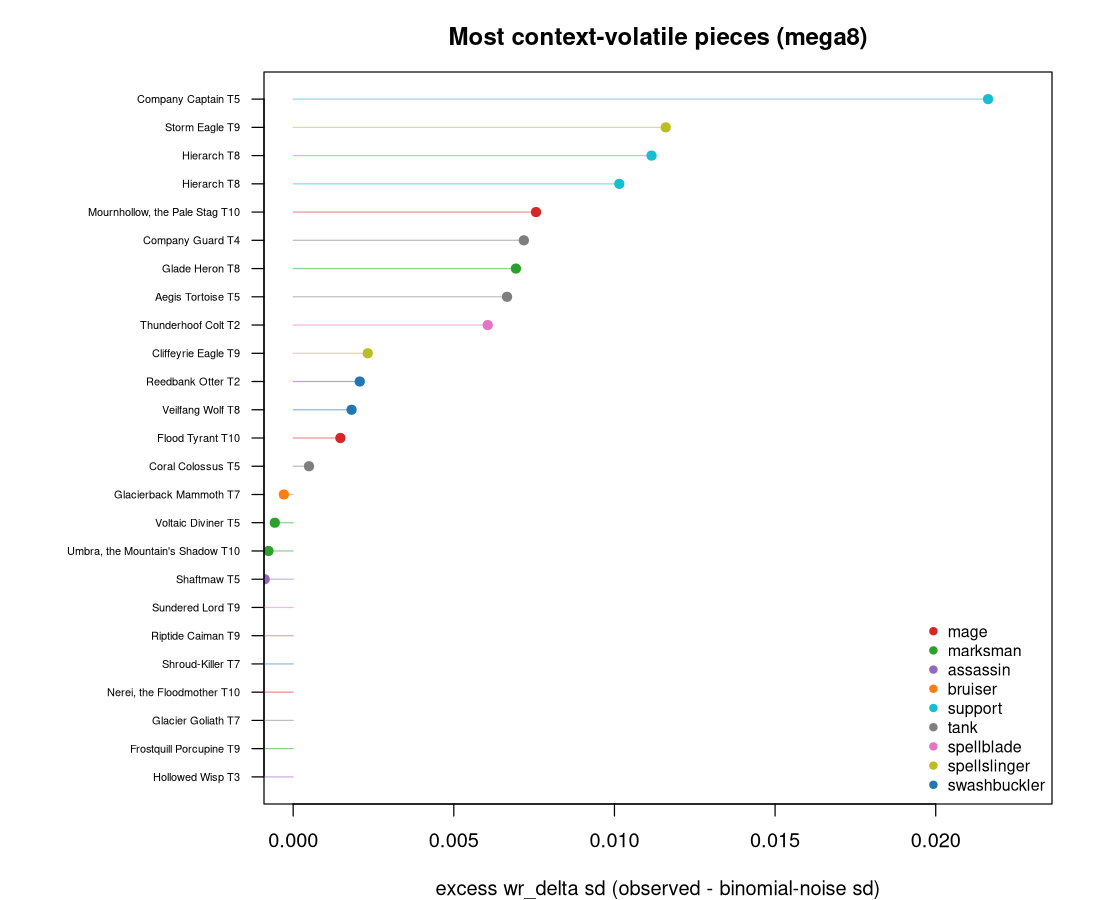
\includegraphics[width=0.86\linewidth,height=0.42\textheight,keepaspectratio]{plots/m8_11_spread_outliers.png}
\caption*{\small Most context-volatile pieces (excess wr\_delta sd beyond noise)}
\end{figure}

\textbf{Spread is almost entirely sampling noise.} Only \textbf{14 of 360} pieces show \texttt{excess\_\allowbreak{}sd > 0}, and the excesses are small ($\leq$0.022):\\

\medskip
\begin{tabularx}{\linewidth}{LLLrLrr}
\toprule
\textbf{name} & \textbf{affinity} & \textbf{role} & \textbf{tier} & \textbf{wd\_pooled} & \textbf{wd\_sd} & \textbf{excess\_sd} \\
\midrule
Company Captain & clear & support & 5 & $-$0.062 & 0.105 & +0.022 \\
Storm Eagle & thunder & spellslinger & 9 & +0.059 & 0.066 & +0.012 \\
Hierarch & clear & support & 8 & $-$0.164 & 0.093 & +0.011 \\
Mournhollow, the Pale Stag & mist & mage & 10 & +0.042 & 0.051 & +0.008 \\
Company Guard & clear & tank & 4 & $-$0.062 & 0.080 & +0.007 \\
Glade Heron & rain & marksman & 8 & +0.046 & 0.062 & +0.007 \\
Aegis Tortoise & clear & tank & 5 & $-$0.029 & 0.088 & +0.007 \\
\bottomrule
\end{tabularx}
\medskip

\textbf{Takeaway:} \texttt{wr\_\allowbreak{}delta} is not meaningfully context-volatile in mega8 --- the outliers worth acting on are the \emph{absolute} ones in \S{}9.2. Hierarch appears on both lists (under-tuned \emph{and} slightly volatile), reinforcing it as a priority. Full table: \texttt{tables/\allowbreak{}m8\_\allowbreak{}spread\_\allowbreak{}outliers.\allowbreak{}csv}.\\

\subsection*{9.4 Problem pieces --- multi-list cross-reference}

Any single list can flag a benign extreme or sampling noise. The robust signal is a piece that lands on \emph{several} lists at once --- and especially one that is both a \textbf{band-breaker} ($|$\texttt{wr\_\allowbreak{}delta}$|>0.10$, \S{}9.2) \emph{and} a category flier (\S{}7, \S{}9.1) or context-volatile (\S{}9.3). That combination means the piece is off-budget \emph{and} stands out against a specific cohort --- the strongest case that it genuinely needs tuning rather than being a statistical artefact. Membership codes: \textbf{WP}=win\_rate$\sim$power flier, \textbf{DP}=wr\_delta$\sim$power flier, \textbf{DR}=wr\_delta$\sim$role flier, \textbf{DT}=wr\_delta$\sim$tier flier, \textbf{AB}=absolute band-breaker, \textbf{SP}=spread/context-volatile. The 18 pieces on $\geq$2 lists (full table: \texttt{tables/\allowbreak{}m8\_\allowbreak{}problem\_\allowbreak{}pieces.\allowbreak{}csv}):\\

{\small
\begin{tabularx}{\linewidth}{lrrclL}
\toprule
\textbf{piece (role)} & \textbf{$\Delta$} & \textbf{wr} & \textbf{\#} & \textbf{lists} & \textbf{pattern / call} \\
\midrule
Springfrog T1/L3 (support) & +0.140 & 0.642 & 5 & WP+DP+DR+DT+AB & \textbf{EB} --- over-scaled T1 kit; the clearest over-tune in the sweep. \\
Hierarch T8/L3 (support) & $-$0.128 & 0.618 & 4 & DR+DT+AB+SP & \textbf{AG} + volatile --- apex support that stalls; barrier helps allies not self. \\
Steam Engineer T4/L3 (mage) & $-$0.114 & 0.377 & 4 & WP+DR+DT+AB & \textbf{DA} --- loses on raw win rate too; under-built mid mage. \\
Mirewarden Toad T7/L3 (tank) & $-$0.105 & 0.565 & 4 & WP+DR+DT+AB & \textbf{AG} --- apex tank grinder. \\
Aurion T10/L3 (spellblade) & $-$0.151 & 0.753 & 3 & DR+DT+AB & \textbf{AG} --- worst piece in the sweep; apex king. \\
Maw of the Drowned T9/L3 (tank) & $-$0.131 & 0.642 & 3 & DR+DT+AB & \textbf{AG} --- durable apex grinder. \\
Stone Warden T10/L3 (tank) & $-$0.124 & 0.728 & 3 & DR+DT+AB & \textbf{AG} --- apex tank grinder. \\
Springfrog T1/L2 (support) & +0.102 & 0.481 & 3 & DP+DR+AB & \textbf{EB} --- same kit over-budget a level down. \\
Borealis T10/L1 (mage) & +0.114 & 0.613 & 3 & WP+DP+AB & Over --- king kit front-loaded at L1. \\
Dredge-Hulk T7/L3 (bruiser) & $-$0.098 & 0.611 & 2 & DR+DT & \textbf{AG} --- apex bruiser grinder. \\
Cliffeyrie Eagle T9/L3 (sslinger) & $-$0.097 & 0.719 & 2 & DT+SP & \textbf{AG} --- apex spellslinger that stalls. \\
Marshghast Boar T7/L3 (bruiser) & $-$0.093 & 0.571 & 2 & WP+DR & \textbf{AG} --- second apex bruiser grinder. \\
Mournhollow T10/L2 (mage) & +0.101 & 0.648 & 2 & AB+SP & Over --- king mage above budget, mildly volatile. \\
Ember Salamander T3/L3 (mage) & +0.077 & 0.599 & 2 & DP+DT & \textbf{EB} --- low-tier mage over budget. \\
Veilfang Wolf T8/L2 (swash) & +0.064 & 0.525 & 2 & DP+SP & Over --- mid swashbuckler above budget. \\
Hierarch T8/L1 (support) & +0.059 & 0.444 & 2 & DP+SP & \textbf{LF} --- the \emph{over} half of Hierarch's level-flip (under at L3). \\
Glade Heron T8/L3 (marksman) & +0.056 & 0.833 & 2 & WP+SP & Strong fast finisher; on-budget, low concern. \\
Coral Colossus T5/L2 (tank) & +0.051 & 0.402 & 2 & DP+SP & Over --- tank above its P5 budget. \\
\bottomrule
\end{tabularx}
}
\medskip

\textbf{The priority tuning set} is the intersection of \textbf{AB} (off-budget) with a category flier --- the ten pieces carrying \texttt{AB} above. They split cleanly by direction and therefore by fix:\\
\begin{itemize}
\item \textbf{UNDER (apex grinders, add closing pressure):} Aurion, Maw of the Drowned, Stone Warden, Hierarch (L3), Mirewarden Toad --- all \textbf{AG}, plus \textbf{Steam Engineer} (\textbf{DA}, needs a raw rebuild, not just a finisher).
\item \textbf{OVER (trim early/king scaling):} Springfrog (L2 \emph{and} L3 --- top of the over list), Borealis (L1 king front-load), Mournhollow (L2 king).
\end{itemize}
\textbf{Hierarch is the standout:} it is the only piece flagged in \emph{both} directions (UNDER at L3 on 4 lists, OVER at L1) --- a clear \textbf{level-flip}, so its fix is re-shaping the per-level curve, not a flat nudge.\\

\section*{10. Roster health index}

Beyond naming outliers, it is worth scoring the \emph{whole} roster with a single health read. The games industry's standard is the \textbf{win-rate band}: a balanced unit should sit near 50\%, and deviation past a threshold flags it for a change. Riot's published champion-balance framework treats $\sim$48/52\% as the weak/strong band and $\sim$45/55\% as ``broken'' for League of Legends.\footnote{Riot Games, \emph{/dev: Champion Balance Framework}, \url{https://nexus.leagueoflegends.com/en-us/2019/05/dev-champion-balance-framework/}.} Two adaptations are needed here. First, raw win rate is power-confounded in a random-draw sweep, so the band is applied to \texttt{wr\_\allowbreak{}delta} (the power-adjusted residual), where 0 is the target. Second, the sim has no pick/ban, so there is no ``Presence'' signal --- but it gains something human telemetry never has: \textbf{every piece is exposed equally} (median 2{,}340 matches), so there is no popularity bias to correct for.\\

\medskip
\begin{tabularx}{\linewidth}{Lr}
\toprule
\textbf{metric} & \textbf{value} \\
\midrule
within $\pm$0.05 \texttt{wr\_\allowbreak{}delta} (tuned) & 84.2\% \\
within $\pm$0.10 (acceptable) & 97.2\% \\
beyond $\pm$0.10 (outlier) & 2.8\% (10 pieces) \\
sd(\texttt{wr\_\allowbreak{}delta}) & 0.039 \\
sd(win\_rate) & 0.114 \\
Gini(win\_rate) & 0.121 \\
\bottomrule
\end{tabularx}
\medskip

\textbf{The roster is healthy by this standard.} Five sixths of all pieces are tightly on-budget and the residual sd (0.039) is a quarter of the raw win-rate sd (0.114) --- i.e. most of the win-rate spread is power doing its job, not mistuning. The low Gini (0.121) of win rate confirms outcomes are not concentrated in a small clique of dominant pieces. The 10 pieces beyond $\pm$0.10 are the \S{}9.2 list, headed by the apex four.\\

\begin{figure}[H]\centering
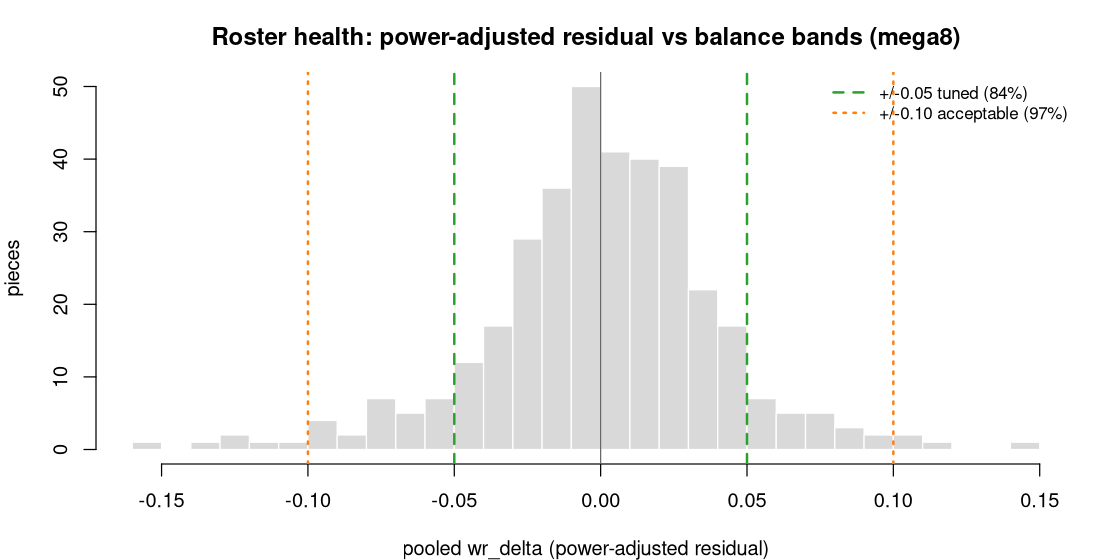
\includegraphics[width=0.86\linewidth,height=0.40\textheight,keepaspectratio]{plots/m8_13_health_band.png}
\caption*{\small Power-adjusted residual distribution against the tuned ($\pm$0.05) and acceptable ($\pm$0.10) bands}
\end{figure}

\section*{11. Combat pacing}

The combined file carries \texttt{mean\_\allowbreak{}duration\_\allowbreak{}ticks} per piece, never used in prior reports. Median fight duration is \textbf{6{,}710 ticks} --- 56\% of the 12{,}000-tick cap --- so the typical battle resolves with comfortable headroom, which is why timeouts are low (\S{}8). Duration is the direct timeout driver (\texttt{cor(duration, timeout)=0.92}, right panel).\\

The pacing--power relationship is the interesting one. The \emph{median} duration is essentially flat across power (L1 6{,}711, L2 6{,}782, L3 6{,}816 ticks --- a 1.5\% spread), but the \textbf{variance fans out sharply at high power}: low/mid-power pieces cluster tightly around 6{,}700 ticks, while high-power L3 pieces spread across the \emph{entire} 4{,}600--8{,}800-tick range. The apex does not resolve at one speed --- it \textbf{splits into fast finishers (close in $<$5{,}500 ticks) and slow grinders (drag past 8{,}000)}. The weak overall \texttt{cor(power, duration)=$-$0.19} is the fast-finisher tail pulling the mean down, not a uniform speed-up.\\

\begin{figure}[H]\centering
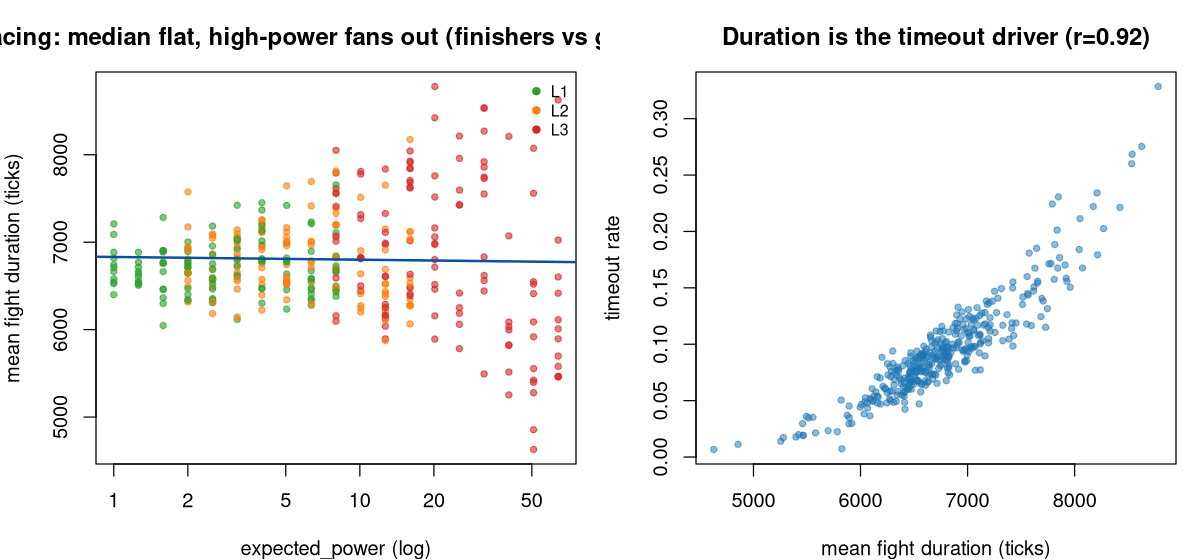
\includegraphics[width=0.96\linewidth,height=0.42\textheight,keepaspectratio]{plots/m8_14_pacing.png}
\caption*{\small Left: duration vs power, coloured by level (median flat, high-power variance fans out). Right: duration drives timeout.}
\end{figure}

\section*{12. Behavioral archetypes (clustering beyond designer roles)}

Win rate alone hides \emph{how} a piece wins. A growing balance-research line argues for clustering units on their \emph{behavioral} signature rather than reading per-unit win rates in isolation.\footnote{See e.g. \emph{Beyond Win Rates: A Clustering-Based Approach to Character Balance Analysis in Team-Based Games}, arXiv:2502.01250; and \emph{Identifying and Clustering Counter Relationships of Team Compositions in PvP Games}, arXiv:2408.17180.} Following that approach, we ran an unsupervised \textbf{k-means clustering} ($k{=}6$) over six standardized outcome features per piece --- win\_rate, \texttt{wr\_\allowbreak{}delta}, timeout\_rate, weather\_sensitivity, duration, and power --- with \emph{no} knowledge of the designer role labels, then asked which roles fall into which cluster.\\

\medskip
\begin{tabularx}{\linewidth}{rrrrrrLr}
\toprule
\textbf{cluster} & \textbf{n} & \textbf{win\_rate} & \textbf{wr\_delta} & \textbf{timeout} & \textbf{power} & \textbf{top role} & \textbf{purity} \\
\midrule
C1 (efficient mid) & 73 & 0.535 & +0.033 & 0.071 & 11.4 & mage & 0.23 \\
C2 (durable grinder) & 15 & 0.607 & $-$0.069 & 0.209 & 33.7 & tank & 0.67 \\
C3 (low-power base) & 168 & 0.423 & $-$0.005 & 0.089 & 4.3 & support & 0.22 \\
C4 (high-power carry) & 24 & 0.701 & $-$0.051 & 0.053 & 44.7 & spellblade & 0.38 \\
C5 (midline wall) & 66 & 0.497 & +0.005 & 0.140 & 10.8 & tank & 0.47 \\
C6 (apex finisher) & 14 & 0.824 & +0.033 & 0.022 & 53.1 & mage & 0.36 \\
\bottomrule
\end{tabularx}
\medskip

\textbf{Finding 1 --- behavior is organised by power and durability, not by designer role.} Cluster purity is low (0.22--0.67): every designer role smears across multiple clusters. The two principal components of the feature space are \textbf{power/strength (PC1, 45\% of variance)} and \textbf{durability/pace (PC2, 29\%)} --- so a piece's outcome signature is set far more by \emph{where it sits on the power curve and how long its fights run} than by its role tag. Roles are a design vocabulary; they are not behaviorally separable in outcome space.\\

\textbf{Finding 2 --- the apex sag is a pacing split, and this is the actionable result.} The high-power pieces divide into two clusters that win very differently: \textbf{C6 ``apex finisher''} (power 53, timeout 0.02, fast, \texttt{wr\_\allowbreak{}delta} \emph{+0.033}) and \textbf{C2 ``durable grinder''} (power 34, timeout 0.21, slow, \texttt{wr\_\allowbreak{}delta} \emph{$-$0.069}). The under-delivery of \S{}7 is concentrated almost entirely in C2 (and the high-power C4 carries, $-$0.051) --- pieces that \emph{grind} toward the tick cap --- while the pieces that close fast are on or above budget. So the apex four (Aurion, Maw of the Drowned, Hierarch, Stone Warden) under-deliver \textbf{because their kits stall the fight, not because their raw numbers are low.} A T.36c fix should add closing/burst pressure, not flat stats.\\

\begin{figure}[H]\centering
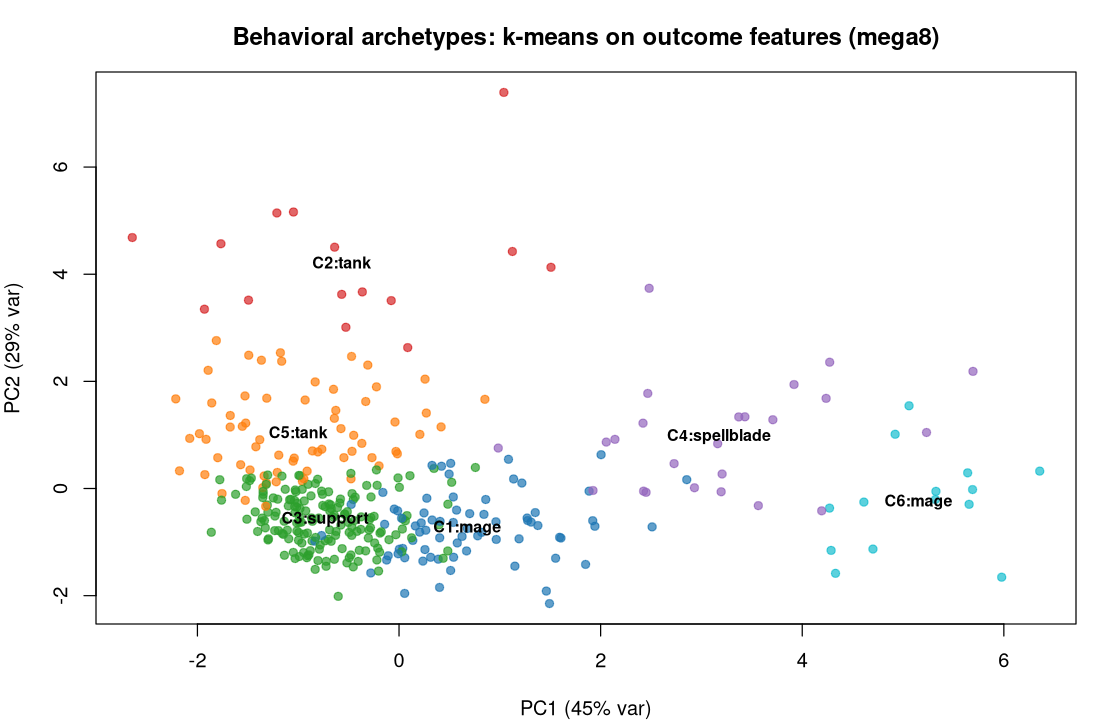
\includegraphics[width=0.90\linewidth,height=0.46\textheight,keepaspectratio]{plots/m8_15_archetypes.png}
\caption*{\small k-means archetypes in outcome-feature PCA space; centroids labelled by dominant designer role. PC1 = power, PC2 = durability/pace.}
\end{figure}

\section*{13. Methodology: mapping to industry balance analytics}

\begin{quotebox}
\textbf{How studios balance from data, and where this sweep sits.}\\[2pt]
\textbf{Win-rate bands (Riot).} The dominant practitioner method: assume a balanced unit wins $\sim$50\%, flag deviation past a band, patch on a cadence. Used here in power-adjusted form (\S{}10).\\[2pt]
\textbf{Latent-strength models (Bradley--Terry / Elo).} Estimate a scalar strength per unit from head-to-head results; the win probability of $i$ over $j$ is a logistic function of their strength difference.\footnote{The Bradley--Terry paired-comparison model is the standard framework for latent strengths from pairwise results.} Our \texttt{expected\_\allowbreak{}wr} power-threshold model is a deterministic cousin; a true Bradley--Terry fit needs the 1v1 matrix (skipped in this sweep --- a candidate for a dedicated 1v1 mega run). These scalar models are known to miss \textbf{non-transitive} (rock-paper-scissors) structure, which motivates the clustering line below.\\[2pt]
\textbf{Counter / archetype clustering.} Recent work clusters compositions by counter-relationship or behavioral signature to expose structure win rates hide (\S{}12).\\[2pt]
\textbf{What the sim has that telemetry lacks.} No pick/ban means no ``Presence'' signal --- but also \textbf{no popularity or skill confound}: every piece is played an equal, large number of times by an identical (deterministic) policy, so a low win rate is never ``unpopular/misplayed,'' it is the kit. And the engine is byte-deterministic, so any finding re-runs exactly. The trade-off: no human meta, no skill-expression axis, and AI policy can under-use a kit a human would exploit --- so treat these as \emph{designer-intent} reads, not live-meta predictions.
\end{quotebox}

\section*{14. Recommendations}

\begin{itemize}
\item \textbf{Apex L3 under-delivery (priority for T.36c) --- fix the \emph{pace}, not the stats.} The four T8--10 L3 pieces \textbf{Aurion, Maw of the Drowned, Hierarch, Stone Warden} under-deliver vs power ($-$0.12 to $-$0.15). The clustering (\S{}12) localises \emph{why}: they belong to the slow ``durable grinder'' archetype that wins by dragging fights toward the tick cap, not the fast ``apex finisher'' archetype which is on-budget. So the fix is \textbf{closing pressure / burst / a finisher mechanic}, not more flat stats --- adding raw power would only deepen the grind. This is the one structural residual left.
\item \textbf{Hierarch specifically.} On both the under-tuned and the context-volatile lists --- the clearest single target.
\item \textbf{Mage deficit: fixed, no action.} The re-axis closed the standing mage problem (\S{}4); mage is now a mild surplus role. Monitor that it does not drift further positive.
\item \textbf{Weather favor: no action.} Working as designed at $\sim$+0.01; the overstating metric bug is fully resolved (0.0\% zero-fill rows).
\item \textbf{Watch the small-format over-performers} (Springfrog, Lostlight Wisp at T1 L3) --- low-tier supports punching above budget. Minor, but the mirror image of the apex sag.
\end{itemize}

\section*{15. Reproducibility}

\begin{lstlisting}
# 1. Run the sweep (workers = CPU cores)
python -m tools.simulation.mega --workers 16 --skip 1v1 \
    --out results/mega/mega8

# 2. Analysis + tables + cache
Rscript reviews/mega_sim/13_mega8.R

# 3. Core figures (m8_01..m8_12)
Rscript reviews/mega_sim/14_mega8_plots.R

# 4. Supplementary analyses (health/pacing/archetypes, m8_13..m8_15)
Rscript reviews/mega_sim/15_mega8_extra.R

# 5. This PDF
xelatex -output-directory=reviews/mega_sim \
    reviews/mega_sim/mega8_analysis_report.tex
\end{lstlisting}

Tables written to \texttt{reviews/\allowbreak{}mega\_\allowbreak{}sim/\allowbreak{}tables/\allowbreak{}m8\_\allowbreak{}*.\allowbreak{}csv}; cache to \texttt{cache\_\allowbreak{}mega8.\allowbreak{}rds}; figures to \texttt{reviews/\allowbreak{}mega\_\allowbreak{}sim/\allowbreak{}plots/\allowbreak{}m8\_\allowbreak{}*.\allowbreak{}png}. The engine is byte-deterministic --- same tree + same flags reproduce the CSVs exactly.\\

\end{document}
